\documentclass[8pt,a4paper]{article}
\usepackage[T1]{fontenc}


%\usepackage[latin1]{inputenc}
%\usepackage[cyr]{aeguill}
\usepackage[francais]{babel}
\usepackage[many]{tcolorbox}

\usepackage[margin=2cm]{geometry}
\usepackage{isabelle,isabellesym}

% further packages required for unusual symbols (see also
% isabellesym.sty), use only when needed

\usepackage{amssymb}
  %for \<leadsto>, \<box>, \<diamond>, \<sqsupset>, \<mho>, \<Join>,
  %\<lhd>, \<lesssim>, \<greatersim>, \<lessapprox>, \<greaterapprox>,
  %\<triangleq>, \<yen>, \<lozenge>

%\usepackage{eurosym}
  %for \<euro>

%\usepackage[only,bigsqcap]{stmaryrd}
  %for \<Sqinter>

%\usepackage{eufrak}
  %for \<AA> ... \<ZZ>, \<aa> ... \<zz> (also included in amssymb)

%\usepackage{textcomp}
  %for \<onequarter>, \<onehalf>, \<threequarters>, \<degree>, \<cent>,
  %\<currency>

% this should be the last package used
\usepackage{pdfsetup}

% urls in roman style, theory text in math-similar italics
\urlstyle{rm}
\isabellestyle{it}

% for uniform font size
%\renewcommand{\isastyle}{\isastyleminor}

\usepackage{amsmath}

%ROLAND
\usepackage{float} %% ROLAND float doit être avant hyperrel pour utiliser [H]
\usepackage{hyperref}
\usepackage{fancyvrb}
\usepackage{amssymb}
\usepackage{amsthm}
\theoremstyle{plain}
\newtheorem{axiome}{Axiome}
\newtheorem*{axiome*}{Axiome}

\newtheorem{postulat}{Postulat}
\newtheorem*{postulat*}{Postulat}

\begin{document}

%\title{IsaGeoCoq: Partial porting of GeoCoq 2.4.0. Case studies: 
%Tarski's postulate of parallels implies the 5th postulate of Euclid, 
%the postulate of Playfair and 
%the original postulate of Euclid.}
\title{IsaGeoCoq2: Géométrie élémentaire - Axiomes de Tarski}
\author{Roland Coghetto\\
  \\
  cafr-msa2p asbl\\
  Rue de la Brasserie 5\\
  7100 La Louvière\\
Belgique}
\maketitle
\begin{abstract}
  La librarie GeoCoq contient
\end{abstract}
\tableofcontents
\section{Introduction}
Cette bibliothèque est construite à partir des axiomes de la géométrie élémentaitaire de Tarski.

La version actuelle s'appelle \textbf{IsaGeoCoq2}.

Elle contient les théories suivantes, réparties en fichiers:
\begin{enumerate}
\item Géométrie neutre dans l'espace: \textbf{Tarski\_Neutral};
\item Géométrie neutre dans le plan: \textbf{Tarski\_2D};
  \item Propriétés de continuité: \textbf{Tarski\_Archimedes};
  \item Equivalence de postulats et axiomes de parallèles: \textbf{Tarski\_Postulate\_Parallels};
  \item Géométrie euclidienne dans l'espace: \textbf{Tarski\_Euclidean};
  \item Géométrie euclidienne dans le plan: \textbf{Tarski\_Euclidean\_2D};
  \item Exercices de géométrie scolaire: \textbf{Highschool1};
    \item Exercices de géométrie scolaire: \textbf{Highschool2}.
  \end{enumerate}

\section{Historique des versions}
Cette version du document est la suite du travail de formalisation \textbf{IsaGeoCoq},
publié dans l'Archive Formal Proofs
\footnote{\url{https://www.isa-afp.org/index.html}} et ayant pour titre
\textit{Tarski's Parallel Postulate implies the 5th Postulate of Euclid,
  the Postulate of Playfair and the original Parallel Postulate of Euclid}
\cite{IsaGeoCoq-AFP}
\footnote{\url{https://www.isa-afp.org/entries/IsaGeoCoq.html}}.

La bibliothèque \textbf{IsaGeoCoq} a été complétement réorganisée: les définitions initiales ont été séparées entre définitions relative à la géométrie neutre et celle relative aux postulats des parallèles.
ont été intégrées dans des théories différentes.

De plus la formalisation de certains équivalences des postulats a été poursuivies et complètée.

Afin de distinguer les deux versions, on appellera la version actuelle \textbf{IsaGeoCoq2}.
\subsection{\textbf{IsaGeoCoq}}
\subsubsection{Résumé}
Le résumé, en français\footnote{La version originale, en anglais, est disponible, sur le site de l'A.F.P:
\url{https://www.isa-afp.org/browser_info/current/AFP/IsaGeoCoq/document.pdf}}
, de la première version:

%\begin{quote}
  La librairie GeoCoq est une formalisation de la géométrie à l'aide de l'assistant de preuve Coq.
  %The GeoCoq library contains a formalization of geometry using the Coq proof assistant.
  Elle contient à la fois des preuves de fondations de géométrie
%It contains both proofs about the foundations of geometry
  \cite{tarski,narboux:inria-00118812,boutry:hal-01483457,narboux:hal-01779452}
  que des résultats de preuves dans le même style que ceux d'une école secondaire
  \cite{beeson:hal-01912024}(Code Repository https://github.com/GeoCoq/GeoCoq).
  %and high-level proofs in the same style as in high-school.
  
  Certains théorèmes sont également inspirés par \cite{tarski} ont aussi été formalisés avec d'autres assistants interactifs de preuve
  (comme Metamath ou Mizar) ou des assistants automatiques de preuve

%Some theorems also inspired by \cite{tarski} are also formalized with others ITP(Metamath, Mizar) or ATP
\cite{sutcliffe1998tptp,dhurdjevic2015automated,beeson2014otter,
stojanovic2010coherent,beeson2017finding,beeson2019proof,
narboux2018computer,boutry2018formalization,
{DBLP:conf/csedu/DoreB18a},
{DBLP:journals/fm/RichterGA14},{DBLP:journals/fm/CoghettoG16},
{DBLP:journals/fm/CoghettoG17},{DBLP:journals/fm/CoghettoG19}}.

Nous avons porté une partie seulement de la bibliothèque \textbf{GeoCoq 2.4.0} grâce à l'assistant de preuve
\textbf{Isabelle/Hol}: plus précisément, les fichiers \verb+chap02.v+ à \verb+Chap13_3.v+, \verb+suma.a+
ainsi que les définitions associés et quelques fichiers utiles pour les démonstrations de certains postulats des parallèles.

%We port a part of the GeoCoq 2.4.0 library within the Isabelle/Hol proof 
%assistant: more precisely, the files Chap02.v to Chap13$\_$3.v, suma.v as 
%well as the associated definitions and some useful files for 
%the demonstration of certain parallel postulates.  

Bien que les démonstrations issues de \textbf{Coq} sont écrites dans un langage procédural
%While the demonstrations in Coq are written in procedural language
\cite{wiedijk2012synthesis},
la retranscription a été effectuée dans le langage déclaratif \textbf{Isar}
%the transcript is done in declarative language Isar
\cite{nipkow2002structured}.

L'approche synthétique des démonstrations a été directement inspirée par les preuves contenues dans GeoCoq.

%The synthetic approach of the demonstrations are directly inspired by 
%those contained in GeoCoq.

Certains démonstrations sont à mettre au crédit de G.E. Martin (<<lemma bet$\_$le$\_$lt:>> in Ch11$\_$angles.thy, prouvé par Martin et noté Theorem 18.17 dans 
\cite{martin2012foundations}) ou de Gupta H.N (comme le \verb+Krippen Lemma+, prové par Gupta dans son travail de thèse (PhD) en 1965 et noté Theorem 3.45).
(voir \cite{gries:hal-01228612}).

%Some demonstrations are credited to G.E Martin(<<lemma bet$\_$le$\_$lt:>> in Ch11$\_$angles.thy, proved by Martin as Theorem 18.17 in 
%\cite{martin2012foundations}) or 
%Gupta H.N (Krippen Lemma, proved by Gupta in its PhD in 1965 as Theorem 3.45).
%(See \cite{gries:hal-01228612}).

Dans ce travail, les preuves ne sont pas constructives.
L'outil \textbf{sledgehammer} a été utilisé pour trouver la plupart des démonstrations ou des énoncés utilisés à l'intérieur des démonstrations.

%In this work, the proofs are not contructive. 
%The sledeghammer tool being used to find some demonstrations.

Les noms des lemmes et théoèmes ont été conservés, dans la mesure du possible, ainsi que les noms des définitions.

%The names of the lemmas and theorems used are kept as far as possible 
%as well as the definitions.

Quand les noms étaient déjà utilisés dans \textbf{Isabelle/Hol} ou bien que certains caractères n'étaient pas valides d'un assistant de preuve à l'autre,
une traduction différente a été proposée.
Ainsi \verb+Len+ a été traduit par \verb+TarskiLen+ et \verb+anga'+ dans \verb+Ch13_angles.v+ par \verb+angaP+.

Pour certains définitions, l'ordre de mise en évidence de certains variables a été modifiée (cf. \verb+Midpoint+, \verb+Out+, \verb+Inter+,\dots).

%A different translation has been proposed when the name was already used in 
%Isabel/Hol ("Len" is translated as "TarskiLen") or that characters were not 
%allowed in Isabel/Hol ("anga'" in Ch13$\_$angles.v is translated as "angaP").
%For some definitions the highlighting of a variable has changed the order or 
%the position of the variables (Midpoint, Out, Inter,...).

Tous les lemmes sont valides dans les espaces de Tarski avec les axiomes de la géométrie absolue (neutre).

%All the lemmas are valid in absolute/neutral space defined with Tarski's axioms.

Il est à noter que T.J.M. Makarios \cite{Tarskis_Geometry-AFP} avait commencé
la démonstration de certains propositions, principalement
ceux des chapitres 2 et 3 \cite{tarski}. Il a utilisé des définitions qui sont légèrement différentes
de celles utilisées dans GeoCoq ainsi que dans ce travail.
Par exemple, Makarios a introduit l'axiome \verb+A11+ (Axiome de continuité) dans la définition de
\verb+Tarski_absolute_space+.


%It should be noted that T.J.M. Makarios \cite{Tarskis_Geometry-AFP} has 
%begun some demonstrations of certain proposals
%mainly those corresponding to SST chapters 2 and 3.
%It uses a definition that does not quite coincide with the definition 
%used in Geocoq and here. As an example, Makarios introduces 
%the axiom A11 (Axiom of continuity) in the definition of the locale 
%"Tarski$\_$absolute$\_$space". 

De plus, la définition de \verb+TarskiAbsolute+ de l'article \textit{Poincaré Disc Model}\footnote{\url{https://www.isa-afp.org/entries/Poincare_Disc.html}}
\cite{PoincareDisc,Poincare_Disc-AFP} n'est pas identique à la définition de \verb+Tarski_neutral_dimensionless+ de GeoCoq.

%Furthermore, the definition of the locale "TarskiAbsolute" \cite{PoincareDisc,Poincare_Disc-AFP} is not 
%not identical to the one defined in the "Tarski$\_$neutral$\_$dimensionless" 
%class of GeoCoq.

En effet, celui-ci ne contient pas l'axiome \verb+upper_dimension+.
Dans certains cas, il convient d'utiliser cet axiome.
Il est alors ajouté le suffixe \verb+_2D+ dans la fichier pour indiquer sa présence.

%Indeed this one does not contain the axiom "upper$\_$dimension". In some cases
%particular, it is nevertheless to use the axiom "upper$\_$dimension". 
%The addition of the word "$\_$2D" in the file indicates its presence.

Dans la dernière partie, il est formalisé que, dans le cadre de la géométrie neutre (absolue),
les postulats de Playfair, du 5\ieme postulat d'Euclide et le postulat originel d'Euclide sont conséquences de 
l'axiome des parallèles de Tarski.

Ces démonstrations, ici non constructives, sont directement inspirées du travail de 
\cite{gries:hal-01228612,boutry:hal-01178236}.

%In the last part, it is formalized that, in the neutral/absolute space, the axiom of the parallels of the system of Tarski 
%implies the Playfair axiom, the 5th postulate of euclide and the postulate
%original from Euclid.
%These proofs, which are not constructive, are directly inspired by 
%\cite{gries:hal-01228612,boutry:hal-01178236}.
%\end{quote}
\subsubsection{Contenu}


Cette bibliothèque
contient 4 définitions concernant les parallèles:

On utilise indistinctement les mots ``axiome'' et ``postulat''.

Dans la suite, on utilise le langage naturel suivant:
\begin{itemize}
\item On note par $A-B-C$, pour signaler que le point $B$ est sur le \textit{segment} $[A,C]$. $A$ peut être identique à $C$.
  Le point $B$ peut coïncider avec l'une des extrémités $A$ ou $C$, voire les deux.
  
\item On note par $AB$, la droite passant par les deux points distincts $A$ et $B$;
\item On note par $A_1A_2\parallel B_1B_2$, les droites $A_1A_2$ et $B_1B_2$ sont parallèles.
\item On note par $P \in AB$, que les points $P$, $A$ et $B$ sont alignés.
 
\end{itemize}
On utilise un pseudo-code suivant:

\begin{tabular}{|c|c|c|}
  \hline
  Pseudo-code & & Isabelle code \\
  \hline
  \verb+<forall>+ & $\forall$ & \verb+\<forall>+ \\
  \verb+<and>+ & $\wedge$ & \verb+\<and>+\\
  \verb+<noteq>+ & $\neq$ & \verb+\<noteq>+\\
  \verb+<exists>+ & $\exists$ & \verb+\<exists>+\\
  \verb+<implies>+ & $\rightarrow$ & \verb+\<longrightarrow>+ \\
  \verb+<not>+ & $\lnot$&\verb+\<not>+\\
  \verb+<equiv>+ & $\Longleftrightarrow$ & \verb+\<equiv>+ \\
  \verb+<or>+ & $\lor$ & \verb+\<or>+\\
  \hline
  
\end{tabular}

  \begin{enumerate}
  \item Tarski's parallel postulate
  \item Euclid 5
  \item Euclid's parallel postulate
  \end{enumerate}


  \subsubsection{Quelques définitions}
Nous ne reprenons dans cette section que des définitions utiles pour comprendre les postulats présentés ci-dessous.

Les notations suivantes sont adoptées\footnote{Pour des raisons de compatibilités,
nous utiliserons les notations présentes dans, par exemple,
\textit{Parallel postulates and continuity axioms: a mechanized study in intuitionistic logic using Coq} de Boutry, Gries, Narboux et Schreck
(voir \cite{boutry2019parallel})}
 :

\begin{tabular}{|l|l|l|}
  \hline
  IsaGeoCoq Notation & GeoCoq Notation & Notation \\
  \hline
  \verb+Bet A B C+ & \verb+Bet A B C+ & $A - B - C$ \\
  &&B est entre A et C\\
    \hline
    \verb+BetS A B C+ & \verb+Bet A B C+ & $A \vdash B \dashv C$ \\
    && B est distinct de A et de C et B est \\
    && entre A et C \\
    \hline
    
  \verb+Cong A B C D+ & \verb+Cong A B C D+ & $A B \equiv C D$ \\
  &&Les segments $\overline{AB}$ et $\overline{CD}$ sont congruents\\
    \hline

  \verb+Col A B C+ &\verb+Col A B C+ &$Col A B C$ \\
  &&A,B et C sont alignés \\
  \hline
  
  \verb+Col A B C <and>+ & \verb+Col A B C <and>+ &A est un point de la ligne BC\\
  \verb+B <noteq> C+ &  \verb+<not> B = C+ &$A \in BC$\\

    \hline

    \verb+<not> Col A B C <and>+ & \verb+<not> Col A B C <and>+ \\
    \verb+B <noteq> C+ & \verb+<not> B = C+&$A \not\in BC$\\
    &&A n'est pas un point de la ligne BC\\
    \hline

  \verb+Coplanar A B C+ &\verb+Coplanar A B C D+ &$Cp A B C D$ \\
  &&A,B,C et D sont coplanaires\\
    \hline

  \verb+A B ParStrict C D+ &\verb+Par_strictA B C D + &$A B \parallel_{s} C D$ \\
  &&les droites AB et CD sont strictement \\
  &&parallèles\\
    \hline

  \verb+A B Par C D+ &\verb+Par A B C D+ &A B $\parallel$ C D \\
  &&les droites AB et CD sont parallèles\\
    \hline

  \verb+A B TS C D+ & \verb+TS A B C D+ & $-A - B- \frac{\ \ C\ }{\ D\ \ }$ \\
  &&C et D sont de part et d'autre de la droite AB \\
    \hline

  \verb+A B OS C D+ & \verb+OS A B C D+ & $-A - B - \frac{\ C \ D \ }{} $ \\
  &&C et D sont du même côté de la droite AB \\
    \hline

  \verb+A B C D E F SumA G H I+& \verb+SumA A B C D E F G H I+ & $A B C \widehat{+} D E F \widehat{=} G H I$ \\
  &&la somme des angles $\angle A B C$ et $\angle D E F$ \\
  && est égale à l'angle $\angle G H I$\\
  \hline
  
  \verb+SAMS A B C D E F+& \verb+SAMS A B C D E F+ & $A B C \widehat{+} D E F \widehat{\leq} \widehat{2\perp}$ \\
  &&la somme des angles $\angle A B C$ et $\angle D E F$ \\
  && est inférieur ou égal à deux angles droits\\
  \hline

    \verb+A B C CongA D E F+& \verb+ CongA A B C D E F+ & $A B C \widehat{=} D E F$ \\
  &&les angles $\angle A B C$ et $\angle D E F$ \\
  && sont congruents\\
  \hline

\end{tabular}

\begin{tcolorbox}
\begin{verbatim}
  <forall> A B C. BetS A B C 
<equiv>
  Bet A B C <and> A <noteq> B <and> B <noteq> C
\end{verbatim}
\end{tcolorbox}
Dans la suite, on utilisera indistinctement les notations \verb+BetS A B C+ ou $A \vdash B \dashv C$.

\begin{tcolorbox}
\begin{verbatim}
  <forall> A B C. Col A B C 
<equiv>
  Bet A B C <or> Bet A C B <or> Bet C A B
\end{verbatim}
\end{tcolorbox}
Dans la suite, on utilisera indistinctement les notations \verb+Col A B C+ ou $A,B,C \text{sont alignés}$.
\begin{tcolorbox}
\begin{verbatim}
  <forall> P A B . P Out A B 
<equiv>
A <noteq> P <and> B <noteq> P <and> 
(Bet P A B <or> Bet P B A)
\end{verbatim}
\end{tcolorbox}

\begin{tcolorbox}
\begin{verbatim}
<forall> A B P Q.
A B TS P Q <equiv>
<not>Col P A B <and> <not> Col Q A B <and>
<exists> T. (Col T A B <and> Bet P T Q)
\end{verbatim}
\end{tcolorbox}

    \begin{figure}[H] %[ht!]
  \centering
    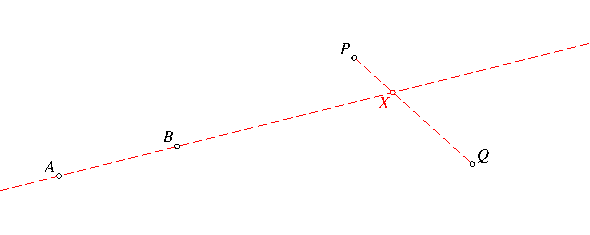
\includegraphics[width=90mm]{fig07.pdf}
\caption{A B TS P Q - Espace euclidien de dim. 2\label{TS1}}
\end{figure}


Il est possible de comprendre \verb+TS+ comme \textit{two side}.
\begin{tcolorbox}
\begin{verbatim}
  <forall> A B P Q.
 A B OS P Q <equiv>
<exists> R. A B TS P R <and> A B TS Q R
\end{verbatim}
\end{tcolorbox}
Il est possible de comprendre \verb+OS+ comme \textit{one side}.

    \begin{figure}[H] %[ht!]
  \centering
    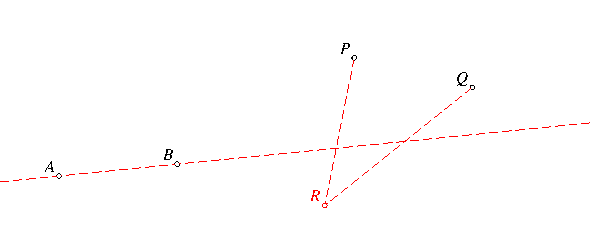
\includegraphics[width=90mm]{fig08.pdf}
\caption{A B OS P Q - Espace euclidien de dim. 2\label{OS1}}
\end{figure}


\begin{tcolorbox}
\begin{verbatim}
<forall> A B C D E F.
A B C CongA D E F <equiv>
  A <noteq> B <and> C <noteq> B <and> D <noteq> E <and> F <noteq> E <and>
<exists> A' C' D' F'.
(Bet B A A' <and> Cong A A' E D <and> Bet B C C' <and> 
Cong C C' E F <and> Bet E D D' <and> Cong D D' B A <and>
 Bet E F F' <and> Cong F F' B C <and> Cong A' C' D' F')
\end{verbatim}
\end{tcolorbox}

    \begin{figure}[H] %[ht!]
  \centering
    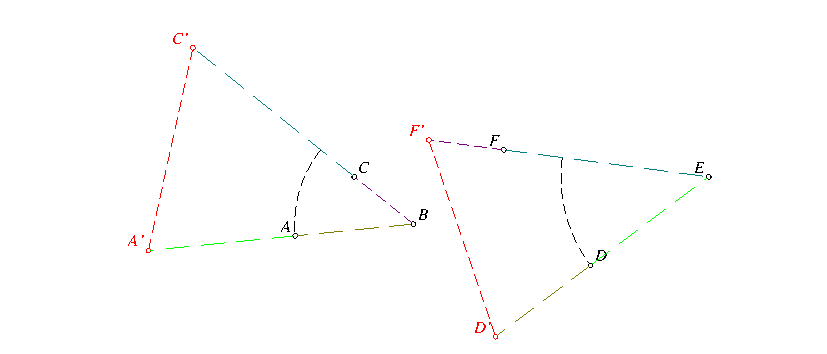
\includegraphics[width=150mm]{fig09.pdf}
\caption{CongA A B C D E F - Espace euclidien de dim. 2\label{CongA1}}
\end{figure}


\begin{tcolorbox}
\begin{verbatim}
<forall> A B C D.
Coplanar A B C D <equiv>
<exists> X. 
  ((Col A B X <and> Col C D X) <or>
   (Col A C X <and> Col B D X) <or>
   (Col A D X <and> Col B C X))
\end{verbatim}
\end{tcolorbox}

  \begin{figure}[H] %[ht!]
  \centering
    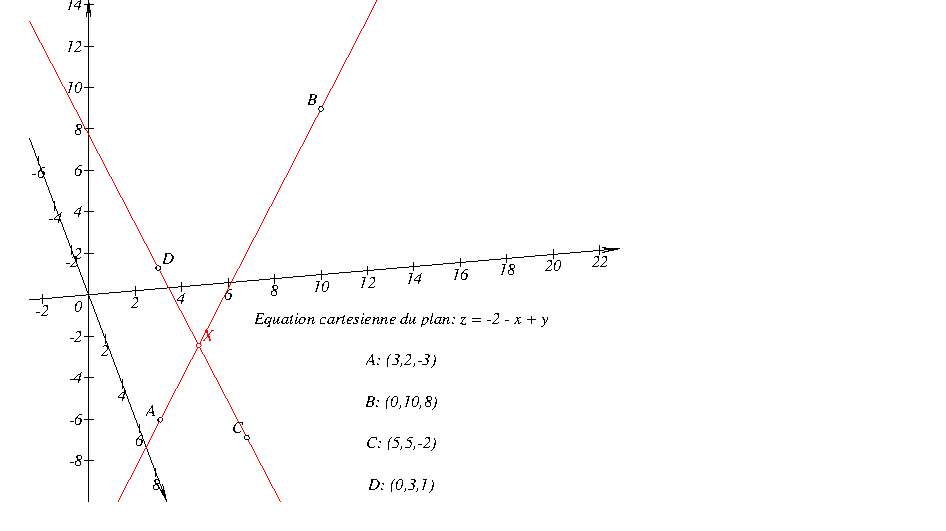
\includegraphics[width=150mm]{fig05.pdf}
\caption{Coplanar A B C D - Espace euclidien de dim. 3 - Version 1\label{Coplanar1}}
\end{figure}

    \begin{figure}[H] %[ht!]
  \centering
    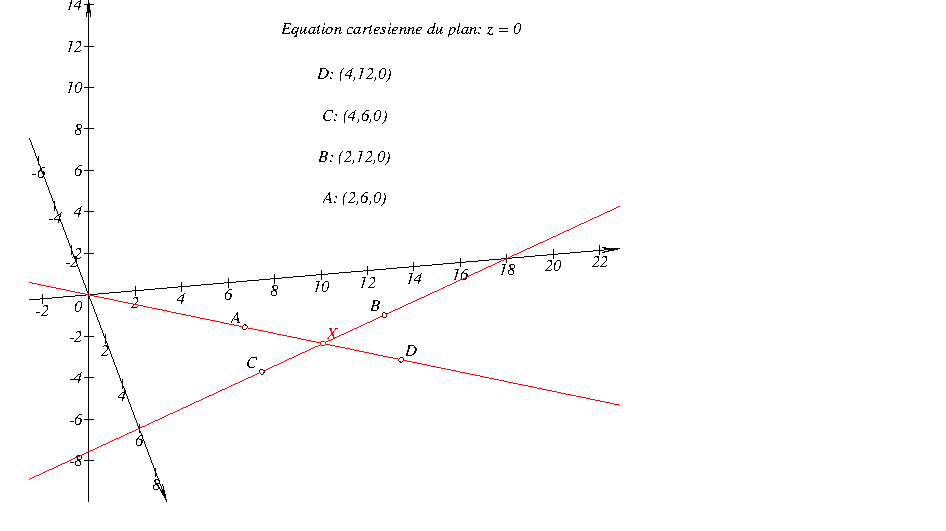
\includegraphics[width=150mm]{fig06.pdf}
\caption{Coplanar A B C D - Espace euclidien de dim. 3 - Version 2\label{Coplanar2}}
\end{figure}

\begin{tcolorbox}
\begin{verbatim}
<forall> A B C D E F.
  SAMS A B C D E F <equiv>
A <noteq> B <and> (E Out D F <or> <not> Bet A B C) <and>
<exists> J. (C B J CongA D E F <and> 
             <not> B C OS A J  <and> 
             <not> A B TS C J  <and> 
             Coplanar A B C J)
\end{verbatim}
\end{tcolorbox}

    \begin{figure}[H] %[ht!]
  \centering
    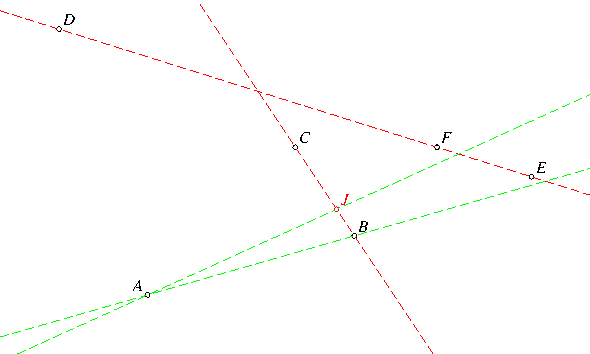
\includegraphics[width=100mm]{fig10.pdf}
\caption{SAMS A B C D E F\label{SAMS}}
\end{figure}

    
    \begin{figure}[H] %[ht!]
  \centering
    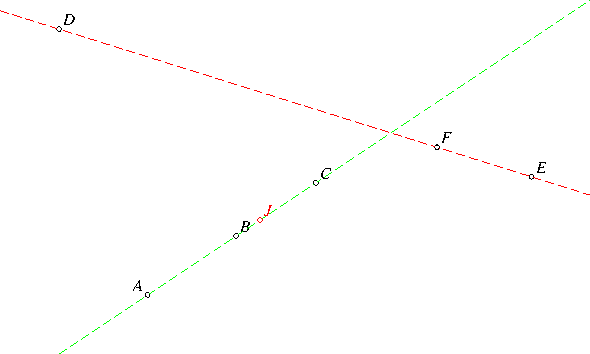
\includegraphics[width=100mm]{fig11.pdf}
\caption{SAMS A B C D E F - Version Bet A B C\label{SAMS2}}
\end{figure}

        \begin{figure}[H] %[ht!]
  \centering
    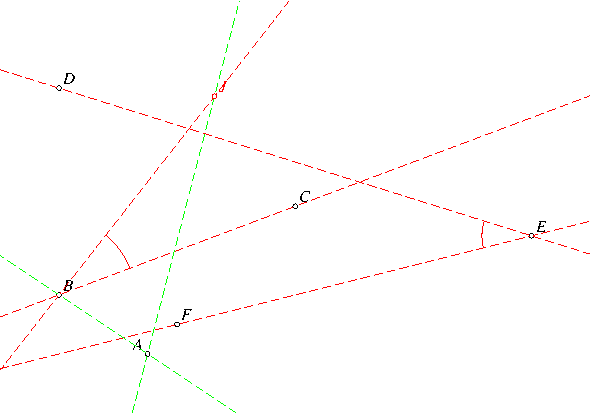
\includegraphics[width=100mm]{fig12.pdf}
\caption{SAMS A B C D E F - Version <not> Bet A B C\label{SAMS3}}
\end{figure}

\begin{tcolorbox}
\begin{verbatim}
 <forall> A B C D E F G H I.

A B C D E F SumA G H I <equiv>

<exists> J. (C B J CongA D E F <and> 
             <not> B C OS A J <and> 
             Coplanar A B C J <and> 
             A B J CongA G H I)"
\end{verbatim}
\end{tcolorbox}

\subsubsection{L'axiome des parallèles de Tarski}

  \begin{postulat}[L'axiome des parallèles de Tarski (Tarski's parallel postulate)]
    Si $A - D - T$, $B -D -C$ et $A \neq D$ alors
    il existe deux points $X$ et $Y$ tels que $A - B - X$, $A -C-Y$ et $X-T-Y$.
  \end{postulat}
  \begin{tcolorbox}
\begin{verbatim}
  <forall> A B C D T.
     Bet A D T <and> Bet B D C <and> A <noteq> D 
<implies>
     (<exists> X Y. Bet A B X <and> Bet A C Y <and> Bet X T Y)
\end{verbatim}
  \end{tcolorbox}
  \begin{figure}[H] %[ht!]
  \centering
    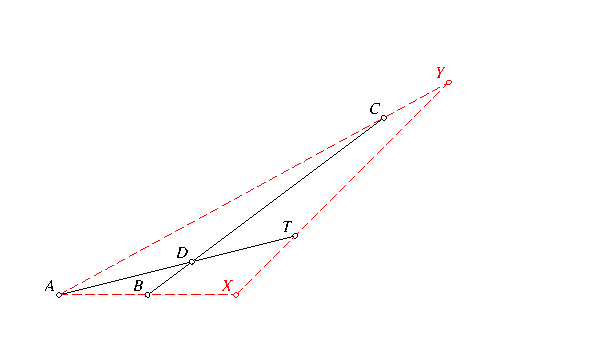
\includegraphics[width=90mm]{fig01.pdf}
\caption{Tarski's parallel postulate\label{TarskiParallelPostulate}}
\end{figure}

  Tim Makarios a montré ce résultat avec \textbf{Isabelle/Hol} dans son travail
\textit{The independence of Tarski's Euclidean axiom}
\cite{Tarskis_Geometry-AFP}
dans le fichier \verb+Euclid_Tarski.thy+ :
  \begin{figure}[H] %[ht!]
  \centering
    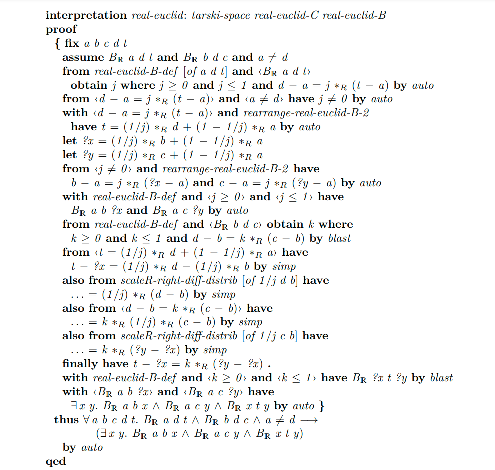
\includegraphics[width=150mm]{MakariosAxiom10.pdf}
\caption{Tarski's parallel postulate - Makarios version\label{TarskiParallelPostulateMakarios}}
\end{figure}


  
John Harisson l'a également montré, à l'aide de \textbf{Hol/Light}\footnote{\url{https://github.com/jrh13/hol-light/blob/master/100/independence.ml}}: 
\begin{verbatim}
(* Independence of the parallel postulate. The statement and some ideas are  *)
(* taken from Tim Makarios's MSc thesis "A mechanical verification of the    *)
(* independence of Tarski's Euclidean axiom".                                *)
(*                                                                           *)
(* In the file Multivariate/tarski.ml it is shown that all 11 of Tarski's    *)
(* axioms for geometry hold for the Euclidean plane `:real^2`, with          *)
(* betweenness and congruence of segments as:                                *)
(*                                                                           *)
(*      B x y z  <=> between y (x,z)                                         *)
(*      ab == pq <=> dist(a,b) = dist(p,q)                                   *)
\end{verbatim}
Plus précisément\footnote{\url{https://github.com/jrh13/hol-light/blob/master/Multivariate/tarski.ml}},
\begin{verbatim}
(* ------------------------------------------------------------------------- *)
(* Axiom 10 (Euclidean axiom).                                               *)
(* ------------------------------------------------------------------------- *)

let TARSKI_AXIOM_10_EUCLIDEAN = prove
 (`!a b c d t:real^N.
        between d (a,t) /\ between d (b,c) /\ ~(a = d)
        ==> ?x y. between b (a,x) /\ between c (a,y) /\ between t (x,y)`,
  REPEAT GEN_TAC THEN GEOM_ORIGIN_TAC `a:real^N` THEN REPEAT STRIP_TAC THEN
  MP_TAC(ISPECL [`vec 0:real^N`; `d:real^N`; `t:real^N`]
        BETWEEN_EXISTS_EXTENSION) THEN
  ASM_REWRITE_TAC[LEFT_IMP_EXISTS_THM; VECTOR_ARITH
   `d + u % (d - vec 0):real^N = (&1 + u) % d`] THEN
  X_GEN_TAC `u:real` THEN STRIP_TAC THEN
  MAP_EVERY EXISTS_TAC [`(&1 + u) % b:real^N`; `(&1 + u) % c:real^N`] THEN
  ASM_REWRITE_TAC[between; dist; GSYM VECTOR_SUB_LDISTRIB] THEN
  ASM_REWRITE_TAC[VECTOR_SUB_LZERO; NORM_NEG;
                  VECTOR_ARITH `b - (&1 + u) % b:real^N = --(u % b)`] THEN
  ASM_SIMP_TAC[NORM_MUL; REAL_LE_ADD; REAL_POS; real_abs] THEN
  REWRITE_TAC[GSYM REAL_ADD_LDISTRIB; REAL_EQ_MUL_LCANCEL] THEN
  ASM_REWRITE_TAC[GSYM dist; GSYM between] THEN REAL_ARITH_TAC);;
\end{verbatim}

Adam Grabowski a montré dans \verb+GTARSKI2.MIZ+\cite{DBLP:journals/fm/CoghettoG16} que
  cet axiome est satisfait dans le plan euclidien $\mathbb{R}^2$:
\begin{verbatim}
::$N Axiom of Euclid
theorem :: GTARSKI2:47  :: Axiom A10 -- Axiom of Euclid
  for a,b,c,d,t being Element of TarskiEuclid2Space st
    between a,d,t & between b,d,c & a <> d holds
      ex x,y being Element of TarskiEuclid2Space st
        between a,b,x & between a,c,y & between x,t,y;
\end{verbatim}
Plus précisément:
\begin{verbatim}
theorem AxiomA10: :: Axiom A10 -- Axiom of Euclid
  for a,b,c,d,t being Element of TarskiEuclid2Space st
    between a,d,t & between b,d,c & a <> d holds
      ex x,y being Element of TarskiEuclid2Space st
        between a,b,x & between a,c,y & between x,t,y
  proof
    let a,b,c,d,t be Element of TarskiEuclid2Space;
    assume that
A1: between a,d,t and
A2: between b,d,c and
A3: a <> d;
G0: Tn2TR d in LSeg(Tn2TR a, Tn2TR t ) by A1,ThConv6;
    set v = Tn2TR a, w = Tn2TR t;
    consider jj being Real such that
G2: 0 <= jj & jj <= 1 & Tn2TR d = (1-jj)*v + jj*w by RLTOPSP1:76,G0;
g1: Tn2TR d - Tn2TR a = (1-jj)*v - v + jj*w by RVSUM_1:15,G2
           .= (1-jj + (-1)) * v + jj*w by RVSUM_1:50
           .= jj*w + (jj * (-1))*v
           .= jj*w + jj * ((-1)*v) by RVSUM_1:49
           .= jj * (w - v) by RVSUM_1:51;
    set jt = 1 / jj;
JJ: jj <> 0
    proof
      assume jj = 0; then
      Tn2TR d - Tn2TR a = 0.TOP-REAL 2 by g1,RLVECT_1:10;
      hence thesis by A3,RLVECT_1:21;
    end;
    set xxx = jt * (Tn2TR b - Tn2TR a) + Tn2TR a;
ww: the MetrStruct of TarskiEuclid2Space = the MetrStruct of Euclid 2 by
      GTARSKI1:def 13; then
    reconsider xx = xxx as Element of TarskiEuclid2Space by EUCLID:22;
    jj * (xxx - Tn2TR a) =
      jj * (jt * (Tn2TR b - Tn2TR a) + (Tn2TR a - Tn2TR a)) by RLVECT_1:28
      .= jj * ((1 / jj) * (Tn2TR b - Tn2TR a) + 0.TOP-REAL 2) by RLVECT_1:15
      .= (jj * (1 / jj)) * (Tn2TR b - Tn2TR a) by RLVECT_1:def 7
      .= 1 * (Tn2TR b - Tn2TR a) by XCMPLX_0:def 7,JJ
      .= Tn2TR b - Tn2TR a by RVSUM_1:52; then
    Tn2TR b in LSeg (Tn2TR a, Tn2TR xx) by G2,ThConvAGI; then
T1: between a,b,xx by ThConv6;
    set yyy = jt * (Tn2TR c - Tn2TR a) + Tn2TR a;
    reconsider yy = yyy as Element of TarskiEuclid2Space by ww,EUCLID:22;
    jj * (yyy - Tn2TR a) = jj * (jt * (Tn2TR c - Tn2TR a) +
      (Tn2TR a - Tn2TR a)) by RLVECT_1:28
      .= jj * (jt * (Tn2TR c - Tn2TR a) + 0.TOP-REAL 2) by RLVECT_1:15
      .= (jj * jt) * (Tn2TR c - Tn2TR a) by RLVECT_1:def 7
      .= 1 * (Tn2TR c - Tn2TR a) by XCMPLX_0:def 7,JJ
      .= (Tn2TR c - Tn2TR a) by RVSUM_1:52; then
    Tn2TR c in LSeg (Tn2TR a, Tn2TR yy) by G2,ThConvAGI; then
T2: between a,c,yy by ThConv6;
    Tn2TR d in LSeg (Tn2TR b, Tn2TR c) by A2,ThConv6; then
    consider kk being Real such that
Y1: 0 <= kk & kk <= 1 & Tn2TR d - Tn2TR b = kk * (Tn2TR c - Tn2TR b)
      by ThConvAG;
    jt * (Tn2TR d - Tn2TR a) = (1 / jj) * jj * (Tn2TR t - Tn2TR a)
      by g1,RLVECT_1:def 7
        .= 1 * (Tn2TR t - Tn2TR a) by JJ,XCMPLX_0:def 7
        .= Tn2TR t - Tn2TR a by RVSUM_1:52; then
w1: jt * (Tn2TR d - Tn2TR a) + Tn2TR a =
      Tn2TR t + (- Tn2TR a + Tn2TR a) by RLVECT_1:def 3
                  .= Tn2TR t + 0.TOP-REAL 2 by RLVECT_1:5;
W2: Tn2TR yy - Tn2TR xx =
      (1 / jj) * (Tn2TR c - Tn2TR a) + Tn2TR a -
        Tn2TR a - (1 / jj) * (Tn2TR b - Tn2TR a)
        by RLVECT_1:27
      .= jt * (Tn2TR c - Tn2TR a) + (Tn2TR a - Tn2TR a) -
        (1 / jj) * (Tn2TR b - Tn2TR a)
        by RLVECT_1:28
      .= jt * (Tn2TR c - Tn2TR a) + 0.TOP-REAL 2 -
        (1 / jj) * (Tn2TR b - Tn2TR a)
        by RLVECT_1:15
      .= jt * ((Tn2TR c - Tn2TR a) - (Tn2TR b - Tn2TR a)) by RLVECT_1:34
      .= jt * (Tn2TR c - Tn2TR b) by ThWW;
    Tn2TR t - Tn2TR xx = jt * (Tn2TR d - Tn2TR a) + Tn2TR a -
      Tn2TR a - (1 / jj) * (Tn2TR b - Tn2TR a)
         by RLVECT_1:27,w1
      .= jt * (Tn2TR d - Tn2TR a) + (Tn2TR a - Tn2TR a) -
        (1 / jj) * (Tn2TR b - Tn2TR a)
         by RLVECT_1:def 3
      .= jt * (Tn2TR d - Tn2TR a) + 0.TOP-REAL 2 - (1 / jj) *
        (Tn2TR b - Tn2TR a) by RLVECT_1:5
      .= jt * ((Tn2TR d - Tn2TR a) - (Tn2TR b - Tn2TR a)) by RLVECT_1:34
      .= jt * (Tn2TR d - Tn2TR b) by ThWW
      .= jt * kk * (Tn2TR c - Tn2TR b) by RLVECT_1:def 7,Y1
      .= kk * (Tn2TR yy - Tn2TR xx) by W2,RLVECT_1:def 7; then
    Tn2TR t in LSeg (Tn2TR xx, Tn2TR yy) by Y1,ThConvAGI; then
    between xx,t,yy by ThConv6;
    hence thesis by T1,T2;
  end;
\end{verbatim}

La bibliothèque \textbf{GeoCoq} contient les résultats suivants dans le fichier \verb+POF_to_Tarski.v+.
%\footnote{A noter que betS a b c implique ($a \neq b$ et $b \neq c$).
%Voir:
%\begin{verbatim}
%\verb+Definition betR a b c := ratio (b - a) (c - a).+ et

%\verb+Definition betS a b c (r := betR a b c)+
%\verb+:=[ \&\& b - a == r *: (c - a), 0 < r \& r < 1].+
%\end{verbatim}
%}


%SUPER
\begin{verbatim}
Lemma euclid' a b c d t (k1 := betR a d t) (k2 := betR b d c) :
  betS a d t -> bet b d c ->
  exists x y, bet a b x /\ bet a c y /\ bet x t y.
\end{verbatim}

\begin{verbatim}
Lemma euclid a b c d t (k1 := betR a d t) (k2 := betR b d c) :
  bet a d t -> bet b d c -> b <> d -> d <> c ->
  ~ (bet a b c \/ bet b c a \/ bet c a b) ->
  exists x y, bet a b x /\ bet a c y /\ bet x t y.
\end{verbatim}

Plus précisement, avec les définitions suivantes:
\begin{verbatim}
Definition betR a b c := ratio (b - a) (c - a).

Definition betS a b c (r := betR a b c) :=
  [ && b - a == r *: (c - a), 0 < r & r < 1].
\end{verbatim}
on a les preuves:
\begin{verbatim}
Lemma euclid' a b c d t (k1 := betR a d t) (k2 := betR b d c) :
  betS a d t -> bet b d c ->
  exists x y, bet a b x /\ bet a c y /\ bet x t y.
Proof.
case: (b =P c)=> [-> betS_adt|/eqP bc_neq betS_adt bet_bdc].
  by rewrite bet_xax=> /eqP ->; exists t, t; rewrite bet_xxa /bet betS_adt orbT.
set x:=extension a b k1; set y:=extension a c k1; exists x, y.
have: (t == extension a d k1); [|move/betSP: betS_adt =>[_ k1_gt0 k1_lt1]].
  move: betS_adt; rewrite betS_neq12 /betS /betR=> /andP[/andP[/eqP ? _] ?].
  by apply /eqP; rewrite /k1 /betR extensionP.
by move=> /eqP t_def; rewrite !extension_bet // t_def /x /y euclid'_aux.
Qed.

Lemma euclid a b c d t (k1 := betR a d t) (k2 := betR b d c) :
  bet a d t -> bet b d c -> b <> d -> d <> c ->
  ~ (bet a b c \/ bet b c a \/ bet c a b) ->
  exists x y, bet a b x /\ bet a c y /\ bet x t y.
Proof.
move=> /orP[/betEP[[->->]|->|->] b2 _ _ H|]; try solve[by apply bet_colF in H];
[exists b,c|move=> b1 b2 _ _ _]; by [rewrite !bet_axx|move: b2; apply euclid'].
Qed.
\end{verbatim}

%  \fbox{
%    \begin{minipage}[]{10cm}
%$\forall A B C D T.$ Bet $A, D, T \wedge $ Bet $B, D, C \wedge A \neq D
%      \longrightarrow \exists X Y.$ Bet $A, B, X \wedge $Bet $ A,C,Y \wedge $Bet $X, T,Y$
%    \end{minipage}
%    }
\subsubsection{Le 5\ieme postulat d'Euclide}

  \begin{postulat}[Le 5\ieme axiome d'Euclide (Euclid\_5)]
Si $P\vdash T\dashv Q$,
$R\vdash T\dashv S$,
$Q\vdash U \dashv R$, $S \not\in PQ$,

%$\lnot \text{Col} (P, Q, S)$,

$P T \equiv Q T$ et $R T \equiv S T$, alors
il existe un point $I$ tel que $S\vdash Q \dashv I$ et $P \vdash U \dashv I$.
\end{postulat}

Initialement, nous avons la condition $\lnot \text{Col} (P,Q,S)$ mais étant donné que $P\vdash T\dashv Q$,
on a $P \neq Q$, ainsi il suffit d'avoir $S \not\in PQ$.

\begin{tcolorbox}
\begin{verbatim}
   <forall> P Q R S T U.
     BetS P T Q <and> BetS R T S <and> BetS Q U R <and> 
     (<not> Col P Q S) <and> Cong P T Q T <and> Cong R T S T
<implies>
     (<exists> I. BetS S Q I <and> BetS P U I)
\end{verbatim}
  \end{tcolorbox}
  \begin{figure}[H] %[ht!]
  \centering
    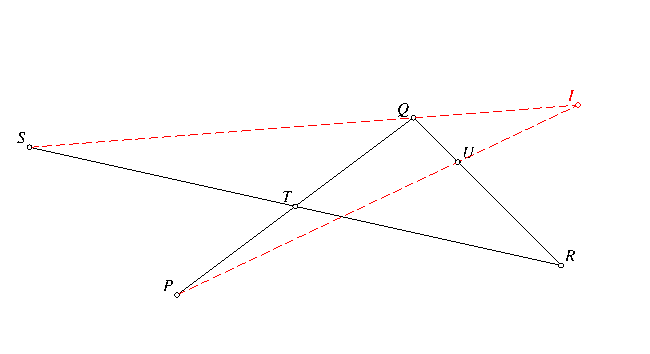
\includegraphics[width=90mm]{fig02.pdf}
\caption{Euclid 5\label{Euclid5}}
\end{figure}

  \subsubsection{Le postulat des parallèles d'Euclide}
  \begin{postulat}[Postulat des parapllèles d'Euclide (Euclid's parallel postulate]
    Si une droite coupe deux autres droites en déterminant deux angles internes
    dont la somme est différente de deux angles droits,
    alors les deux droites se coupent dans le demi-plan
    pour lequel la somme est inférieure à deux angles droits.
  \end{postulat}
  C'est l'énoncé tiré de wikipédia\cite{frwiki:188096497}.
  \begin{tcolorbox}
\begin{verbatim}
  <forall> A B C D P Q R.
     B C OS A D <and> SAMS A B C B C D <and> A B C B C D SumA P Q R <and>
    <not> Bet P Q R 
<implies>
     (<exists> Y. B Out A Y <and> C Out D Y)
\end{verbatim}
  \end{tcolorbox}
  
  \begin{figure}[H] %[ht!]
  \centering
    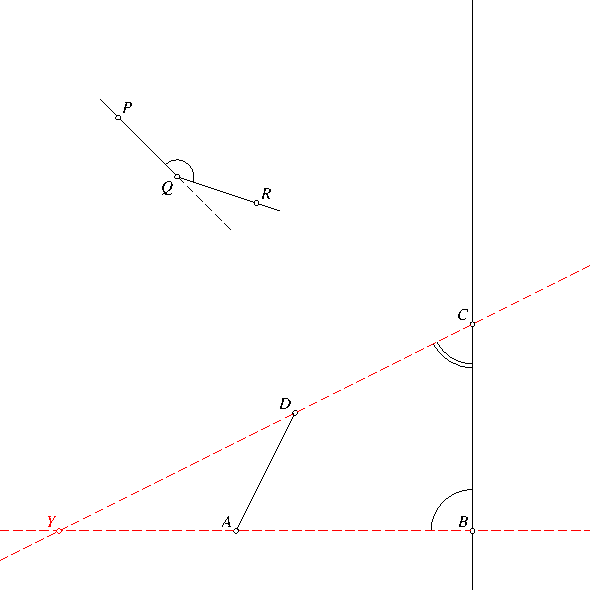
\includegraphics[width=90mm]{fig04.pdf}
    \caption{Euclid's parallel postulate\label{EuclidParallelPostulate}}
  \end{figure}

\subsubsection{Playfair's parallel postulate}
\begin{postulat}[Postulat de Playfair (Playfair's parallel postulate)]
  Par un point donné, on peut mener une et une seule parallèle à une droite donnée.
\end{postulat}
La condition \verb+A B Par C D+, implique que $A \neq B$ et $C\neq D$\footnote{ROLAND: à vérifier}.
  \begin{tcolorbox}
\begin{verbatim}
  <forall> A1 A2 B1 B2 C1 C2 P.
     A1 A2 Par B1 B2 <and> Col P B1 B2 <and> 
     A1 A2 Par C1 C2 <and> Col P C1 C2 
<implies>
     Col C1 B1 B2 <and> Col C2 B1 B2
\end{verbatim}
  \end{tcolorbox}

  \begin{figure}[H] %[ht!]
  \centering
    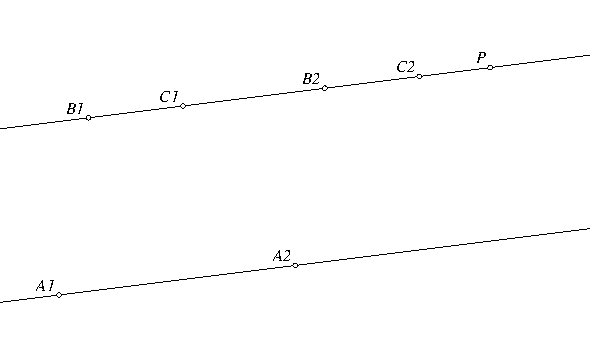
\includegraphics[width=90mm]{fig03a.pdf}
    \caption{Playfair's parallel postulate\label{Playfair1}}
  \end{figure}
      Comme il n'est pas requis que les droites $A_1A_2$ et $B_1B_2$ (ainsi que $A_1A_2$ et $B_1B_2$) soient strictement parallèles, la situation peut-être assez simple:
  \begin{figure}[H] %[ht!]
  \centering
    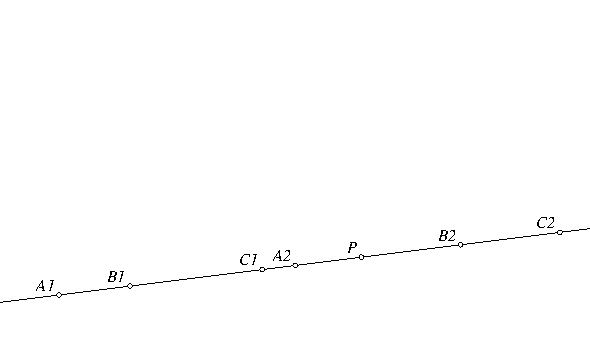
\includegraphics[width=90mm]{fig03b.pdf}
\caption{Playfair's parallel postulate - Cas ligne unique\label{Playfair2}}
\end{figure}

  
    %\fbox{
    %  \begin{minipage}[]{10cm}
    Si $A_1A_2\parallel B_1B_2$ et si $A_1A_2\parallel C_1C_2$,
      si $P \in B_1B_2$ et $P \in C_1C_2$ alors 
      $C_1 \in B_1B_2$ et $C_2\in B_1B_2$
%    \end{minipage}
   % }

  
%    \begin{tcolorbox}[enhanced,ams align,drop fuzzy shadow,
%  colback=yellow!10!white,colframe=yellow!50!black]
%   Si A_1
%  (A_1 A_2 \parallel B_1 B_2 \wedge
%  Col P B_1 B_2 \wedge
%  A_1 A_2 \parallel C_1 C_2 \wedge
%  Col P C_1 C_2
%    \longrightarrow
%    (Col C_1 B_1 B_2 \wedge Col C_2 B_1 B_2)
%    \end{tcolorbox}
%  \end{enumerate}
  Dans le cadre de la géométrie neutre, les théorèmes suivants sont prouvés:
  \begin{enumerate}
   \item Euclid 5 $\longrightarrow$ Euclid's parallel postulate
   \item Tarski's parallel postulate $\longrightarrow$ Euclid 5
   \item Tarski's parallel postulate $\longrightarrow$ Euclid's parallel postulate
   \item Tarski's parallel postulate $\longrightarrow$ Playfair's parallel postulate
  \end{enumerate}

 De façon générale, il est utilisé \verb+smt+ 147 fois pour l'ensemble de cette bibliothèque.


\subsection{\textbf{IsaGeoCoq2}}


La formalisation a été poursuivie avec l'introduction des autres définitions des postulats.
Au total, cette bibliothèque en contient une trentaine.
Il est montré l'équivalence de ces 30 postulats.

%La bibliothèque \textbf{IsaGeoCoq2} a été développée afin de

\textbf{IsaGeoCoq2} apportent les modifications suivantes à la bibliothèque précédente.
\begin{itemize}
\item L'équivalence des 30 postulats associés à \textit{l'unicité des parallèles}.
  Les théorèmes sont contenus dans la théorie \textbf{Tarski\_Postulate\_Parallels.thy};
\item Les propositions obtenues dans un contexte de géoémtrie euclidienne sont rassemblées dans la théorie \textbf{Tarski\_Euclidean};
\item Certains résultats concernant les espaces typiquement de dimensions 2, sont pour ceux valides dans une géoémtrie neutre, contenu dans la théorie \textbf{Tarski\_2D},
  tandis que ceux plus spécifiquement valides dans un plan euclidien sont rassemblés dans la théorie \textbf{Tarski\_Euclidean\_2D}.
\item Enfin, certaines propositions sont reprises comme exercices, dans les deux théories \textbf{Higschool1} et \textbf{Highscool2}.

  Il est à noter que les démonstrations utilisant \verb+smt+ ont été retranscrites en \verb+metis+ ou \verb+meson+, pour la plupart.
  \end{itemize}




% sane default for proof documents
\parindent 0pt\parskip 0.5ex

\clearpage
% generated text of all theories
\input{session}

% optional bibliography
\clearpage
\bibliographystyle{abbrv}
\bibliography{root}

\end{document}

%%% Local Variables:
%%% mode: latex
%%% TeX-master: t
%%% End:
